%%%%%%%%%%%%%%%%%%%%%%%%%%%%%%%%%%%%%%%%%
% Programming/Coding Assignment
% LaTeX Template
%
% This template has been downloaded from:
% http://www.latextemplates.com
%
% Original author:
% Ted Pavlic (http://www.tedpavlic.com)
%
% Note:
% The \lipsum[#] commands throughout this template generate dummy text
% to fill the template out. These commands should all be removed when 
% writing assignment content.
%
% This template uses a Perl script as an example snippet of code, most other
% languages are also usable. Configure them in the "CODE INCLUSION 
% CONFIGURATION" section.
%
%%%%%%%%%%%%%%%%%%%%%%%%%%%%%%%%%%%%%%%%%

%----------------------------------------------------------------------------------------
%	PACKAGES AND OTHER DOCUMENT CONFIGURATIONS
%----------------------------------------------------------------------------------------

\documentclass{article}

\usepackage{fancyhdr} % Required for custom headers
\usepackage{lastpage} % Required to determine the last page for the footer
\usepackage{extramarks} % Required for headers and footers
\usepackage[usenames,dvipsnames]{color} % Required for custom colors
\usepackage{graphicx} % Required to insert images
\usepackage{listings} % Required for insertion of code
\usepackage{courier} % Required for the courier font
\usepackage{multirow}
\usepackage{hyperref}

% Margins
\topmargin=-0.45in
\evensidemargin=0in
\oddsidemargin=0in
\textwidth=6.5in
\textheight=9.0in
\headsep=0.25in

\linespread{1.1} % Line spacing

%----------------------------------------------------------------------------------------
%	CODE INCLUSION CONFIGURATION
%----------------------------------------------------------------------------------------

\definecolor{MyDarkGreen}{rgb}{0.0,0.4,0.0} % This is the color used for comments
\lstloadlanguages{c} % Load Perl syntax for listings, for a list of other languages supported see: ftp://ftp.tex.ac.uk/tex-archive/macros/latex/contrib/listings/listings.pdf
\lstset{language=[sharp]c, % Use Perl in this example
        frame=single, % Single frame around code
        basicstyle=\small\ttfamily, % Use small true type font
        keywordstyle=[1]\color{Blue}\bf, % Perl functions bold and blue
        keywordstyle=[2]\color{Purple}, % Perl function arguments purple
        keywordstyle=[3]\color{Blue}\underbar, % Custom functions underlined and blue
        identifierstyle=, % Nothing special about identifiers                                         
        commentstyle=\usefont{T1}{pcr}{m}{sl}\color{MyDarkGreen}\small, % Comments small dark green courier font
        stringstyle=\color{Purple}, % Strings are purple
        showstringspaces=false, % Don't put marks in string spaces
        tabsize=5, % 5 spaces per tab
        %
        % Put standard Perl functions not included in the default language here
        morekeywords={rand},
        %
        % Put Perl function parameters here
        morekeywords=[2]{on, off, interp},
        %
        % Put user defined functions here
        morekeywords=[3]{test},
       	%
        morecomment=[l][\color{Blue}]{...}, % Line continuation (...) like blue comment
        numbers=left, % Line numbers on left
        firstnumber=1, % Line numbers start with line 1
        numberstyle=\tiny\color{Blue}, % Line numbers are blue and small
        stepnumber=5 % Line numbers go in steps of 5
}

\newcommand{\horrule}[1]{\rule{\linewidth}{#1}}

\newcommand\doubleplus{\ensuremath{\mathbin{+\mkern-10mu+}}}

% Creates a new command to include a perl script, the first parameter is the filename of the script (without .pl), the second parameter is the caption
\newcommand{\perlscript}[2]{
\begin{itemize}
\item[]\lstinputlisting[caption=#2,label=#1]{#1.cs}
\end{itemize}
}

\begin{document}

\begin{tabular}{l l}
\multirow{5}{*}{
\includegraphics[width=2cm]{../../recursos/logo.png}} & Universidad del Istmo de Guatemala \\
 & Facultad de Ingenieria \\
 & Ing. en Sistemas \\
 & Informatica II \\
 & Prof. Ernesto Rodriguez - \href{mailto:erodriguez@unis.edu.gt}{erodriguez@unis.edu.gt} \\
\end{tabular}
\\\\\\

\begin{center}
        \horrule{0.5pt}
        \huge{Laboratorio \#6} \\
        \large{Fecha de entrega: 7 de Marzo, 2019 - 11:59pm} \\
        \horrule{1pt}
\end{center}

\emph{Instrucciones: Resolver cada uno de los ejercicios siguiendo sus respectivas
instrucciones. El trabajo debe ser entregado a traves de Github, en su repositorio del curso, colocado en una carpeta llamada "Laboratorio \#6".
Al menos que la pregunta indique diferente, todas las respuestas a preguntas escritas deben presentarse en
un documento formato pdf, el cual haya sido generado mediante Latex. Este laboratorio
debe ser elaborado en parejas.}

\section*{Tarea \#1 (20\%)}
\label{tarea1}

Un poligono es una figura que esta compuesto de una serie de \emph{vertices}. Todos esos
vertices estan conectados de tal forma que la figura sea cerrada. Por ejemplo, un
triangulo es un poligono con tres puntos y un rectangulo es un poigono de cuatro
puntos. A continuaci\'on se muestran ejemplos de poligonos.
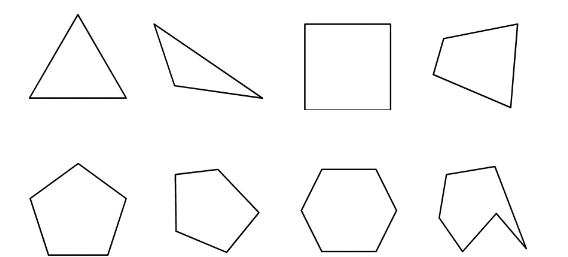
\includegraphics{polygons.png}
\\\\
Su tarea es definir una clase para representar poligonos en espacios de \emph{dos
dimensiones}. Tomar en cuenta que un poligono puede tener una \emph{cantidad arbitraria}
de vertices. Recuerde hacer uso de la \emph{composici\'onn} para separar la complejidad
del problema en varias clases incluyendo una clase llamada ``Vertice'' que se utilize
para representar cada vertice del poligono.
\\\\
La calse \emph{Poligono} debe tener las siguientes caracteristicas:
\begin{itemize}
        \item{Un metodo constructor que acepte una cantidad arbitraria de \emph{vectices}
        como parametros.}
        \item{Debe tener una propiedad que indica el numero de vertices que tiene el
        poligono.}
\end{itemize}

\section*{Tarea \#2 (20\%)}

Existen ocasiones en que un metodo puede no retornar un valor. Un ejemplo es si
se desea saber cual es el quinto vertice de un triangulo, dado que un triangulo
solamente tiene 3 vertices. Para expresar este comportamiento, en C++ se pueden
utilizar \emph{parametros de salida}. Un \emph{parametro de salida} es un parametro
pasado ya sea como referencia o puntero a un metodo. Al finalizar la ejecucion,
el metodo puede actualizar el valor de dicho parametro mediante la asignaci\'on
con el operador igual. El metodo tambi\'en retorna \texttt{true} o \texttt{false}
dependiendo si el metodo retorno un valor o no.
\\\\
Su tarea es implementar el metodo ``$obtenerVertice\ :\ \mathtt{const\ int}\rightarrow\mathtt{Vertice\&}\rightarrow \mathtt{bool}$''.
la cual acepta un numero indicando el vertice que se desea obtener y una referencia a una
instancia de la clase \emph{Vertice}. Si el numero indicado por el parametro corresponde
a un vertice del poligono, este metodo debe asignarle dicho vertice al segundo parametro
y retornar \texttt{true}. De lo contrario, debe retornar \texttt{false}.

\section*{Tarea \#3 (20\%)}

Definir el metodo ``$agregarVertice\ :\ \mathtt{const\ int}\rightarrow \mathtt{const\ Vertice\&}\rightarrow \mathtt{const\ bool}$''
en la clase \emph{Poligono}. Este metodo acepta un entero como parametro y un \emph{Vertice}. Este vertice debe ser agregado
a la lista interna de vertices del poligono. El primer parametro debe estar entre 0 y el numero
de vertices actual de vertices en el poligono de lo contrario el metodo no debe hacer nada
y retornar $\mathtt{false}$. De lo contrario, el vertice debe ser \emph{agregado} en la posici\'on
indicada por el primer parametro. Los vertices que se encuentren despues de este parametro deben
ser desplazados hacia ``atras'' para acomodar el nuevo vertice. Recuerde tambien actualizar
el numero de vertices que tiene el poligono.


\section*{Tarea \#4 (20\%)}
Definir el metodo ``$eliminarVertice\ :\ \mathtt{const\ int}\rightarrow\mathtt{bool}$''. Este
metodo acepta un numero entre 0 y un numero menos que el numero de vertices en este poligono, de
lo contrario, debe retornar $\mathtt{false}$ y no hacer nada. Si el numero esta dentro del
rango permitido, debe eliminar el vertice que se encuentra en esa posici\'on del poligono.
Todos los vertices posteriores al vertice eliminado deben ser movidos para llenar el espacio
que ha quedado. Recuerde actualizar el numeor de vertices en el poligono.

\section*{Tarea \#5 (20\%)}

Definir un metodo {\bf main} el cual debe implementar el flujo definido por
el diagrama a continuaci\'on. Extender el programa y el diagrama con el caso
faltante, el cual corresponde a una opci\'on diferente de 'a','e' o 's':
\\\\
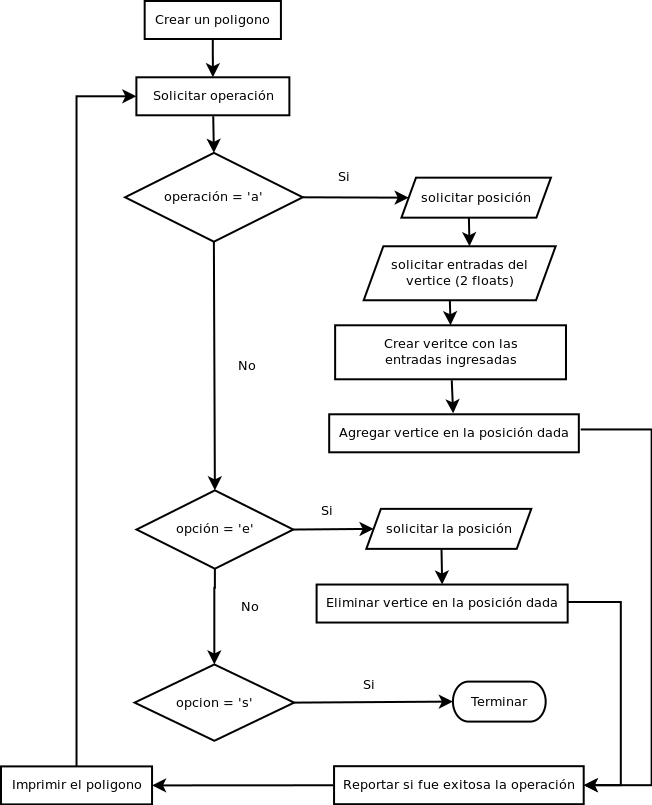
\includegraphics[width=15cm]{flujo.png}

\end{document}